\documentclass[shuuron]{kuee}
\usepackage[dvipdfmx]{graphicx}
\usepackage{kueecite}
\usepackage{url}

\title{心理カウンセリングの品質向上を支援する視覚的分析に関する研究}
\author{上辻智也}
\professor{小山田 耕二 教授}
\course{京都大学工学部}
\department{電気電子工学科 電気工学専攻}
\date{平成30年2月1日}

%%% 本文
\begin{document}
\maketitle
\tableofcontents


%%%序論
\chapter{序論}

現代社会では、多種多様なデータの膨大な量がある。具体的には、様々な会話をもとに分析テキストデータへのニーズが高まってきている。会話テキストのビッグデータに溢れた時代の中で、様々な会話をもとに分析テキストデータへのニーズが高まってきている。

一方で、1991年に日本心身医学会が「心身症とは、身体疾患の中で、その発症や経過に心理社会的因子が密接に関与し、器質的ないし機能的障害が認められる病態をいう。ただし、神経症やうつ病など、他の精神障害に伴う身体症状は除外する」と定義した。そこから心身症はストレスとの深い関連が指摘された病態であると認知され、今日まで広く研究されてきた。心療において,カウンセラーは心身症やストレスからくる身体症状をもつクライエントの治療としてカウンセリングを行う.その中で,カウンセラーはクライエントの関心つまり「対人関係上の問題」に注意を向けて引き出すということがカウンセリングの基本である\cite{zokad}.。

  そこで、心理カウンセリングにおいて、 カウンセラーは、主にストレスの原因による物理的な症状に悩む患者やクライアント(以降、クライエントと統一する)に対してカウンセリングを提供している。カウンセリングの会話記録は音声ないし動画が撮影され、後述するカウンセラー指導・事例検討の目的で役立てられているが、クライエントプライバシーの関係上実際の事例検討やカウンセラー教育の場では、それを手で書き起こした逐語録を用いることが多い。




%%品質の定義


カウンセリングの品質を向上するために事例検討会が行われている。そこでは,熟練のカウンセラーが初心者カウンセラーに指導する機会が設けられている.たとえば今回書き起こしテキストデータを使用した「心療内科における摂食障害専門ヨーガ療法グループ」事例検討会では,初心者カウンセラーに対してカウンセリングに関するアドバイスがなされている.具体的には,クライエントと初心者カウンセラーとのカウンセリング内容を動画で撮影し,その動画書き起こされたカウンセリング内容のテキストデータを,熟練のカウンセラーらが読んで,議論をする,という流れである.そのため,熟練のカウンセラー達が会話の流れを文字で読むだけでは,カウンセリング内容の分析が十分に行えていなかった.

そこで心理カウンセリングの会話書き起こしテキストデータから会話内容を可視化することで、心理カウンセリングの品質向上を支援することができるのではないかと我々は考えた。

ここで、本稿では、「心理カウンセリングの品質向上を支援する視覚的分析」の要素として次の2つについて述べる。
\begin{itemize}
\item 心理カウンセリングにおいて初心者カウンセラーの習熟度の評価を支援する視覚的分析
\item 心理カウンセリングにおいて患者の認知の修正すなわち回復状況の評価を支援する視覚的分析
\end{itemize}



% 本論文では、「カウンセリングの品質向上への支援」を以下のように定義する。
% ・熟練のカウンセラーからのアドバイスを含む、初心者カウンセラーのカウンセリングの質問の品質向上への支援
% ・クライエントの患者の認知の修正をカウンセラーが把握することへの支援

\subsubsection{初心者カウンセラーの習熟度の評価を支援する視覚的分析}



初心者カウンセラーは「対人関係上の問題」を,質問に対する回答としてクライエントから引き出すのに苦戦しているという問題がある.カウンセラーの質問内容については,大きく2種類に分けられている.YesまたはNoで答える質問,または短い言葉だけで答えられるような質問は「閉じられた質問(Closed-ended Question)」または「閉ざされた質問」と呼ばれている.これに対し,クライエントが5W1H「いつ」「どこで」「誰が」「何を」「どのように」「どうした」で答えるような質問は「開かれた質問(Open-ended Question)」と呼ばれている.熟練のカウンセラーによれば,クライエントが何に問題意識を感じているかをカウンセリングで引き出すには,カウンセラーは「閉じられた質問(Closed-ended Question)」よりも「開かれた質問(Open-ended Question)」をしたほうがよいとされている.しかし初心者カウンセラーは「閉じられた質問(Closed-ended Question)」の割合が多く,クライエントが何に問題意識を感じているかをカウンセリングでうまく引き出せないケースが比較的多いとされている.

このように,初心者カウンセラーは「閉じられた質問(Closed-ended Question)」を多く用いる傾向にあるので,熟達カウンセラーは,初心者カウンセラーが「開かれた質問(Open-ended Question)」を自由に使えるように教育したいと考えている.「対人関係上の問題」に注意を向けて引き出すということがカウンセリングの基本であるので,このようにカウンセラーの関心でクライエントを誘導してしまうことはよくないとされている.そのためのチェックが可能になるものが求められている.

カウンセラーの事例検討会において、熟練のカウンセラー達が会話の流れを文字で読むだけでは,カウンセリング内容の分析が十分に行えていなかった.そこで、初心者カウンセラーがどのような質問をして,それによってクライエントからどのような回答を引き出したのか,適切な方法で可視化されることが望まれていた.

そこで本研究では,クライエントと初心者カウンセラーとの会話の流れを,時間軸に沿って可視化するシステムを開発した.本提案システムは熟練のカウンセラーをユーザーとして想定した.熟練のカウンセラーから初心者へのカウンセリング指導において重要なことは,初心者カウンセラーがクライエントにどのような質問を投げかけるかによって,初心者カウンセラーがクライエントからどのような「対人関係上の問題」を引き出したかである.それが一目見てすぐにわかるようになることが,このシステムによって期待されることである.%システムをWeb上に載せることによって,同じ会話データを持っているだけで遠隔のユーザーと同様の可視化を共有することが期待される.



クライエントの会話内容としては,次章で詳しく述べるどの課題領域(仕事,交友,愛)に属するのか,カウンセラーの質問としては,内容が「開かれた質問(Open-ended Question)」なのかまたは「閉じられた質問(Closed-ended Question)」なのかを分類表示できることが必要である.クライエントからの提出した話題が,どの領域に関するものか,カウンセリングの中でその領域がどのように変わっていくかを分析していくと,そのカウンセリングプロセスがより明確になると考える.時系列に沿って見ると,最初にクライエントの関心がどこにあったのか,それに対してカウンセラーからの発話で異なった領域に話題が展開した,というような分析も可能になると考える.

上辻\cite{uetsuji}は会話の流れ可視化システムを開発したが、定量的なユーザー評価を行っておらず、また図形についての比較も不明瞭であった。そこで本稿では
\begin{itemize}
\item 「事例検討会通りに原文を読んでカウンセリングを評価すること」との対比実験
\item 新たなチャート可視化の提案と、既存チャート可視化との対比実験
\end{itemize}
について述べる。

\subsubsection{患者の認知の修正の評価を支援する視覚的分析}

% クライアントは、多くの場合、より多くのクライアントの認知の修正は心理カウンセリングに進行し、「アクションの他人の話をクライアントに自分自身を行っている」。2「彼らが行っていることを行動について話す」の割合として言いる。言い換えれば、「あなた自身の行動を変えるのではなく、相手の行動を変えることに興味がある場合は、認知修正が進んでいる」[1]。したがって、我々は適切なカウンセリングの会話データから、「クライアントの行動」と「クライアントの行動を」分類し、結果を可視化することにより、クライアントの認知の修正の度合いを把握することができる、と考えた。

一連の文章の中から,場面ごとに誰が誰に行動を起こしたか把握したい,会話文や物語の人間関係を想起する必要がある場面がある.たとえば心理カウンセリングにおいて,クライエントは「他人がクライエント自身に行った行動」ではなく,「自分が行った行動」の話をカウンセリング中にする割合が多いほど,患者の治療(以降,これを「認知の修正」と呼ぶ)が進行しているといわれている.心理カウンセリングにおいて, 「相手の行動を変えることより,自分の行動を変えていくことに関心がある方が,認知の修正が進んでいる」[1]とされている.カウンセリングにおける目的は認知の修正であるが,クライエントの回答として「クライエントの身の回りの人の行動」に関する発言よりも「クライエント自身の行動」に関する回答が発せられた方が,クライエントの認知の修正が進行しているとされている.「クライエントの身の回りの人の行動」か「クライエント自身の行動」か,データを可視化することで,クライエントの認知の修正の具合を確認できるのではないかと考えられる.

以上のように,どのような場面で誰が誰に行動したかを文書から抽出することが求められている.それに対し我々は,誰が誰にどのような行動をとったかを時系列で可視化することで,上記のニーズを満足できるのではないかと考えた.このような要求に対し,我々は誰が誰に行動したかという人間関係図を時系列にそった可視化を試みた.


上記の要求に応じて、我々は行動のどのような心理カウンセリング会話中に登場する人々の間で撮影された人間関係のチャートとを組み合わせることの方法で会話データの可視化を試みた。

本論文の構成は次の通りである.第1章は,本論文の序論である.第2章では,本論文の関連研究を挙げる.また,提案システムの開発にあたり必要になってくるカウンセリングの基礎事項について説明する.第3章では,システムの要件を整理した後,本提案システムの設計と実装について述べる.第4章では,提案システムに対する評価として,提案システムからの出力結果の内容とそれに対する考察,ユーザーからのコメントとそれに対する考察,そして本提案システムの抱えている問題点について述べる.第5章では,本論文の結論と本研究が抱える今後の課題について述べる.

%


%
%   特に心理共同でunseling、 カウンセラーは、主にストレスの原因による物理的な症状に心身患者やクライアントとのカウンセリングを提供している。一般的には、初心者カウンセラーは、認知特性とクライアントによる内部問題の難易度回し関心を持っている。
%   初心者カウンセラーは、自分の興味に合わせて心理カウンセリングを続行する傾向があり、および周波数を使用している「クローズド・エンド型の質問(クライアントは答えることができ、 『いいえはい』または『』)」クライアントのために、人の心の中で作成された解釈を確認する。初心者カウンセラーはメイククライアントの認識こだわり答えを得ることができない
% しばしば、初心者カウンセラーのはい/いいえの質問
%   これとは対照的に、専門家のカウンセラーがカウンセリングの内容に関する初心者カウンセラーのための助言に教育訓練の機会を提供する。専門のカウンセラーは、そのため、初心者カウンセラーが「オープンエンドの質問(5W1Hによる質問)」を自由に使用することができる教育する必要がある。しかしながら、 なぜなら、プライバシーの問題のため、専門家は、心理カウンセリングの実際の音声データを取得することはできない。 だから、 いつも監督に、専門カウンセラーは、カウンセリングで音声表記の直接書き起こしテキストと見て、初心者カウンセラーのために誰かを教育する。
%   しかし、書き起こし産物の文書 テキストデータが 心理カウンセリングにおける会話の大規模かつ複雑で、スーパーヴァイザは各データを参照しながら、初心者カウンセラーとクライアント間の特性との会話の状況を抽出することは非常に困難である。この問題を改善するために、我々は、会話データの可視化が有効であると思われることを検討してください。したがって、我々は、初心者カウンセラーによる各質問のためのクライアントの各回答を視覚化するための適切な方法を示すことを検討してください。
%   本研究では、心理カウンセリングに会話の流れを可視化するシステムを提案し、開発した。この提案システムでは、我々はAdlerian心理学の基礎を分類し、各カテゴリグループのためのチャートと時間の経過に沿って分布の変動を可視化表音transcriptio中含まれて、n 心理カウンセリングにいる。本稿では、システムの概要とUの結果を示する専門のカウンセラーによるSER評価。会話の流れの私達の可視化の対象ユーザーは、専門家のカウンセラーである。
%    また、クライアントは、多くの場合、より多くのクライアントの「認知の補正は、」図のように心理カウンセリングに進行し、「アクションの他人の話をクライアントに自分自身を行っている」。2「彼らが行っていることを行動について話す」の割合として言いる。言い換えれば、「あなた自身の行動を変えるのではなく、相手の行動を変えることに興味がある場合は、認知補正が進んでいる」[1]。したがって、我々は適切なカウンセリングの会話データから、「クライアントの行動」と「クライアントの行動を」分類し、結果を可視化することにより、クライアントの認識の変更の度合いを把握することができ、と考えた。
%   上記の要求に応じて、我々は行動のどのような心理カウンセリング会話中に登場する人々の間で撮影された人間関係のチャートとを組み合わせることの方法で会話データを視覚化した。


%%





 

%%%関連研究
\chapter{関連研究}



%%


%%各論文について倍増

  の会話の関連する視覚化のいくつかの作品がある。この章では、我々は、関連する作業を説明し、我々の研究の位置を明らかにした。本研究では、時系列に沿って視覚化方法は、テキストデータを扱う上で重要であると考えている 心理カウンセリングでの会話の流れに。


\section{会話の可視化に関する先行研究}

まず、会話を可視化している先行研究について述べ、それらの先行研究に対しての本研究の位置づけについて説明を行う。会話テキストのビッグデータに溢れた時代の中で、様々な会話をもとに分析テキストデータへのニーズが高まってきている。

Heliangは、Webベースの心理カウンセリングシステム[2]で折れ線グラフと3次元の螺旋構造を持つクライアントのトピックを可視化した。しかし、我々の研究では、ビューの時点で、初心者カウンセラーとクライアントの一対一の会話の流れの可視化と呼ばれる、両方で各発話内容を組み合わせることにより、可視化することが重要である。

  エリック\cite{taskdriven}と技術の二種類で割ったトピックの時間分布のための頂部および底部の非対称層折れ線グラフにより可視化他人。我々の研究では、上部と下部の非対称性の折れ線グラフで絵を描くための可視化技術は、クライアントによって各発話や初心者カウンセラーについて有用であることを考える。しかし、心理カウンセリングの会話の流れを可視化するために、初心者カウンセラーによる質問に対するクライアントのどのような応答を聞くことが重要である。

  伊藤\cite{itoh2010interactive}は、3次元に、ブログのユーザーの興味深いトピックの時系列推移を可視化することができ、システムを開発した。我々の研究では、クライアントによる発話の情報は、時系列、文章のグループ、および文の数によって3次元データから構成されている。他の手で、初心者カウンセラーによって発話の情報を時系列と質問タイプによって2次元データである。しかし、我々はクライアントと初心者カウンセラーとの会話の流れが色分けして2次元のグラフで可視化することができると考えた。

   EL-Assady\cite{el2016contovi}は、スピーカからカテゴリ約トーク量を意味するサイズ文字円、トークカテゴリ円チャートと円とスピーカーパターンを分析するための視覚的な分析手法を開発した。彼らはあなたが話題にしているサークルによって会話を表現する。

しかし、カウンセラーとクライアントのトピック分類が一緒でない限り、彼らの視覚化を使用することはできないので、我々は彼らの視覚化からの質問と回答の間の関係を知ることができない。

  A.タット\cite{tat2002visualising}は、オーディオの可視化を使用し、我々は行動を行動履歴の追加で拡張する方法を示すためにしよう

 これらのパターンの中から、トニー・バーグストローム\cite{bergstrom2007seeing}は、話し手の感情を推測することができるし、どのように彼/彼女が会話中に別のスピーカーに接続されている。しかし、A. Tatおよびトニーは、自然言語の手順を使用して、会話のコンテンツカテゴリを視覚化していないので、我々は彼らの視覚化からの質問と回答の間の関係を知ることができない。

  本研究では、このような問題は心理カウンセリングで初心者カウンセラーによってクライアントから引き出すことができる方法として、これらの発話に対応することが重要である。したがって、我々はクライアントと初心者のカウンセラーによって発話の各情報をことが望ましいと考えた コンパクトシングルチャートで視覚化する。
  ヴァンハムら\cite{van2009mapping}は文章を分析し、そのようなユーザによって指定された「BのA」および「AおよびB」との関係を有向グラフで表現される。接続原因が入力されたテキストデータに現れたときしかし、彼らのシステムから、我々はこれらの言葉が接続されている理由を知っているとすることはできない。

  Tanakaら\cite{tanaka}は効率的に話の内容をリコールインタフェースを開発した。しかし、彼らは文字ではありないものを含め、頻繁キーワードを可視化する。また、彼らはそれがどのようなシーンにあった、方向性、人間関係のどのような種類の部分的な可視化を行っていない。

%%
%
% 会話の可視化に関していくつかの先行研究がある。本章では、関連する研究を説明し、我々の研究の位置づけについて説明する。本研究では、時系列に沿って可視化方法は、心理カウンセリングでの会話の流れテキストデータを扱う上で重要であると考えている。
% Heliang[2]は、Webベースの心理カウンセリングシステムで折れ線グラフと3次元の螺旋構造を用いてクライアントのトピックを可視化した。彼らの研究では,このような多種・多様な心理データを3D グラフで可視化する手法が提案されている.本3D グラフ表示はProcessing プロジェクトを用いて螺旋形状の表示を実
% 現する.また螺旋全体を回転させることで,全体的な傾向や特徴を視覚的に把握することが可能となっている
% 一年間を通じてどのような時期(季節,月)に相談量が多くなっているか,そしてその相
% 談内容の詳細も同時に容易に把握することが可能となっている.
% しかし、我々の研究では、ビューの時点で、初心者カウンセラーとクライアントの一対一の会話の流れの可視化と呼ばれる、両方で各発話内容を組み合わせることにより、可視化することが重要である。
%  エリックと技術の二種類[3]で割ったトピックの時間分布のための頂部および底部の非対称層折れ線グラフにより可視化他人。我々の研究では、上部と下部の非対称性の折れ線グラフで絵を描くための可視化技術は、クライアントによって各発話や初心者カウンセラーについて有用であると考える。しかし、心理カウンセリングの会話の流れを可視化するために、初心者カウンセラーによる質問に対するクライアントのどのような応答を聞くことが重要である。
%  伊藤は、3次元[4]座標上に、ブログのユーザーの興味深いトピックの時系列推移を可視化することができ、システムを開発した。我々の研究では、クライアントによる発話の情報は、時系列、文章のグループ、および文の数によって3次元データから構成されている。他の手で、初心者カウンセラーによって発話の情報を時系列と質問タイプによって2次元データである。しかし、我々はクライアントと初心者カウンセラーとの会話の流れが色分けして2次元のグラフで可視化することが可能であると考えた。
%   EL-Assady [5]は、カテゴリ別にトーク量を意味する円、トークカテゴリを表す円形のチャートを用いて、話者がどのカテゴリのことをしゃべっているかを表す視覚的な分析手法を開発した。彼らはあなたが話題にしているサークルによって会話を表現した。多人数会話の話者行動パターンを分析するための新しい視覚的分析手法として彼らは、会話の主題景観全体にわたる話し手の動きを追跡するためにトピック空間ビューを提案した。彼らのツールは、スピーチの相互作用や行動パターンに関する仮説を生成し、証明するために、政治学者が会話を探るのを支援することを目的としている。関連するテキストの特徴を抽象化するために、スピーカーの一般的な動作や相互作用、時間の経過に伴うインタラクティブな安定した視覚化を探索し、スピーカーの選択に関する詳細な分析を行うためのアニメーション表示を提供している。視覚的沈降法のメタファーを使用することにより、分析者は過去のすべてのスピーカーターンの概要を保持しながら、時間の経過とともに会話の流れの微妙な変化を追跡することができるようになっている。しかし、カウンセラーとクライアントのトピック分類が一緒でない限り、彼らの可視化を使用することは不可能であるので、我々は彼らの可視化方法からの質問と回答の間の関係を知ることが不可能であると考えている。
%  A.タットは、[6]オーディオの可視化を使用し、我々は行動を行動履歴の追加で拡張する方法を示すためにしようとした。
% 
 トニー・バーグストロームの可視化は、[7]話し手の感情を推測することが可能で、どのように彼/彼女が会話中に別の話者に接続されている。しかし、A. Tatおよびトニーは、自然言語の手順を使用して、会話のコンテンツカテゴリを可視化していないので、我々は彼らの可視化からの質問と回答の間の関係を知ることが不可能である。
%  本研究では、このような問題は心理カウンセリングで初心者カウンセラーによってクライアントから引き出すことが可能である方法として、これらの発話に対応することが重要である。したがって、我々はクライアントと初心者のカウンセラーによって発話の各情報をことが望ましいと考えた コンパクトなシングルチャートで可視化することを試みた。
%  カウンセリングについて3.基本的な説明
%  本章で、我々の提案するシステムの開発に必要なカウンセリングの基本的な事項を説明する。Adlerian心理学が提案システム今回の使用データとして扱われるヨガの治療に採用されている。
% ラーと提案システムの設計と実装からのコメントに基づいて可視化システムを開発するための要件について説明する。

\section{カウンセリングの可視化に関する先行研究}

\section{物語の可視化に関する先行研究}

会話書き起こしテキストデータから人間関係図を作り出す研究事例はないが、物語を可視化する事例は人間関係図作成の参考となる。

storyLine\cite{tanahashi2012design} \cite{tanahashi2015efficient}
言語処理を用いていない

自然言語処理を用いた物語の可視化に関する先行研究としては、まずヴァンハム\cite{van2009mapping}らは文章を分析し、そのようなユーザーによって指定された「BのA」および「AおよびB」との関係を有向グラフで表現した。接続詞や前置詞ベースで単語をつなげている彼らのシステムから、我々は誰が誰に対して行動したかを知ることは不可能である。

田中ら\cite{tanaka}は効率的に話の内容を想起できるようなインターフェースを開発した。しかし、彼らは登場人物動詞を線でのみ結んだ無向グラフとして可視化しており、その場面は誰が誰に対して行動したかをそのグラフから把握することはできない。また、彼らの可視化では章ごとのみの可視化となっており、 彼らの可視化を用いてもカウンセラーのどの質問によってカウンセリングの会話の傾向が変わったかを把握することができない。



\section{カウンセリングの基本的事項}
\subsection{カウンセラースーパーヴァイズ}

修論からパクる

% アドラー心理学は、認知行動療法のパイオニアとしてみなされている。あなたがやっていることは、認知の修正であり、同様のアプローチがとられている。アドラー心理学は、オーストリアの精神科医アルフレッド・アドラー(A.アドラー)とその後継[10]によって開発された心理学の理論、思考及び処理技術のシステムである。認知行動療法はそこに来て、実験システムおよび臨床システムはかなり現代までの大まかな流れであると言われている、一緒に参加している。アドラーは、人生のすべての問題は、3つの主要なタスクに分類することが可能である」と述べ、それは、仲間の仕事、仕事のタスク、愛と家族の課題である[11] 生命タスクでAdlerian心理学、 の関係から、表のように永久的な、運命1.:質問者のための親和性、研究タスク:非常任人間関係、友情のタスク:持続性が、運命をやっていない人間関係、愛と家族の仕事。人間関係の問題を取得するのに役立ちる。「任意」(人間関係についての発言をしない)分類理にかなっている。人間関係の物語の中で3つのカテゴリで、それらにあまり動かない人と判断することが可能であるカウンセリングは、より深く、患者から悪い感情の原因を導き出すことが可能である。臨床的観点から臨床的に三つに任意の人間の問題を分類することが非常に有効であるといわれている。

我々の提案の会話の流れの可視化の前手順を 上記分類方法に基づいている。本研究では、時間軸に沿って可視化は、との会話の流れを可視化 クライアント とカウンセラーし、会話の流れが開発したカウンセラーのWebシステムによって発行された質問によってどのように変化するかを明確にしている。

一方、クライアントの認知修正の分析は、何らかの形でのように述べた行動クライアントのカテゴリを使用 図。2 動作は、クライアントの周りの人々が行っていたものが挙げられる。 鎌田\cite{kamata2002}は、 カウンセラーの行動や感情を重要な役割は、クライアントが自己決意と自己責任を取ると不当に他人に介入することなく、他者との協力関係を形成することが可能であるようにクライアントを奨励することである。そのため、不当に他人の行動や感情に介入することなく、クライアント自身の行動や感情を見つけることが重要である。

図

提案した可視化システムの4前の手順
 この章で、我々は詳細に専門のカウンセ

 臨床的観点からは、三つのカテゴリーに人間の問題を分類するために極めて有効であると考えられる。上記分類方法から、我々は次のサブセクションで提案されたシステム、設計および実装するための要件のextrbehaviorを説明する。
\subsection{クライアントの分析}

今回取り扱うテキストデータに記載されているカウンセリングはヨーガ療法を用いている。ヨーガ療法における病理論は、約2800年前に記されたとされる「タイッティリーヤ・ウパニシャッド」に記されている、人間を五層に分けて考える「人間五臓説」にもとづいている\cite{kimura}。マンジュナート\cite{manjunath}は、変化する無常なるものを普遍的なものと錯覚する「理智の誤り」、すなわち「認知の誤り」(これ以降、本論文では「認知」と統一して記す)を基準として、病気について
\begin{itemize}
\item 「認知の誤り」から生じない感染症や外傷などの病気
\item 「認知の誤り」から生じる心身病などの病気
\end{itemize}
の2つにわけている。後者は現代心身医学のストレス認知的評価説
% (Lazarus, Folkman 1984)
\cite{Lazarus}とほぼ一致してると言える\cite{Darshana}。


 % カウンセリングで、「自分の行動を変えるのではなく、相手の行動を変えることに興味がある人は、認知を修正するに進んでいる」と言われている。ときに、クライアントの答え「クライアント自身の行動」ではなく答えるクライアントの認識の修正が進んでいると言われて、 『クライアントの周りの人々の行動を。』

 我々は、または「クライアント自身の行動」「クライアントの周りの人の行動」のデータを可視化することにより、クライアントの知覚の状態を確認可能であることを考えた。一方、我々は年代順に会話内容をテキストで行動の対象と述語を可視化することにより、上記のニーズを満たすことが可能であると考えた。このようなニーズに応えて、我々は行動の対象とオブジェクトの情報を含む人間関係チャートの時系列を可視化してきた。



%%%本提案システム
%%%%%%%%%%%%%%3章%%%%%%%%%%%%%%3%%%%%%%%%%%%%%3%%%%%%%%%%%%%%3
\chapter{カウンセラー習熟度評価支援システム}





第1章で述べた仮説のうち、〜〜を検証するために、我々は会話の流れを可視化するシステムを開発した。本章では、本稿で述べる提案システムの1つである会話の流れ可視化システムの開発、および有効性の検証について述べる。
\section{目的}

本章では,ユーザーである熟練のカウンセラーからのコメントをもとにした提案システム要件抽出,および本提案システムの設計や実装について詳しく述べる.なお本システムでは,クライエントまたはカウンセラーの1発言を,話者の交代によって判断するものとする.つまり,クライエントの1発言は,カウンセラーが喋り終わってクライエントが喋り始めてから,クライエントが喋り終わってカウンセラーが喋り始めるまでである.また,カウンセラーの1発言は,クライエントが喋り終わってから,あるいはカウンセラーが話を切り出し始めてから,カウンセラーが喋り終わってクライエントが喋り始めるまでである.



様々な心理学の学派・セラピーが各カウンセリングに用いられているが、それらの差異にかかわらず、臨床現場でのカウンセリングの初動は、

\begin{enumerate}
 \item インテーク面接による情報取集
 \item その情報に基づいたアセスメント
 \item 上記のアセスメントに従った介入目標の設定とその達成方法の立案
 \item それらの説明と合意をとるインフォームドコンセント
\end{enumerate}
という一連の流れが含まれている。しかし初心者カウンセラーは、上記4項目の中でもまず初めの
\begin{enumerate}
 \item インテーク面接による情報取集
\end{enumerate}
でつまずいてしまうことが多い。情報収集技術には大きく分けて次の2種類の質問がある。
\begin{itemize}
\item 開かれた質問
\item 閉じられた質問
\end{itemize}
・
・


Ivey,A.E.\cite{ivey}のマイクロカウンセリングで示されている「開かれた質問(Open-ended Question)」と「閉じられた質問(Closed-ended Question)」を利用する。特に、「開かれた質問(Open-ended Question)」は情報収集を行っていくうえで特に重要で、5W1Hで質問することで、クライエント自身に答えを考え出してもらうことで、クライエント側の関心について知ることができる。                                                                            

 一般的には、初心者カウンセラーは、認知特性とクライアントによる内なる問題に対して関心を傾注することが困難になる傾向がある。

初心者カウンセラーはこの2つの質問のうち、特に「閉じられた質問(Closed-ended Question)」を必要以上に多く使ってしまう傾向があると言われている。これは

\begin{itemize}
\item 初心者カウンセラー自身の思い込みが先行している
\item クライエントについて十分理解できていない
\end{itemize}
ことを示している。その理由は、初心者カウンセラーが多用する「閉じられた質問(Closed-ended Question)」は、初心者カウンセラーが自身の関心でつくりあげたクライエントの像を確認したために使われているからである。初心者カウンセラーが自身の関心でつくった仮説をそのまま信じることで、クライエントの症状を初心者カウンセラーがその仮説の中に閉じ込めようとしてしまう。

それに対して、熟練のカウンセラーは「開かれた質問(Open-ended Question)」と「閉じられた質問(Closed-ended Question)」を会話の流れに応じて使い分けることで、クライエントの自身に対する洞察を支援し、クライエント自身が気づいていけるようにかかわっていく。これがカウンセラーにもできるようになるためには、カウンセラー自身が客観視を会得して、クライエント自身の関心にカウンセラーが関心を向け、クライエントが発した発言を丁寧に取り扱っていくことが可能になる必要がある。

そこで現在、スーパーヴァイズ
しかし現状 
どうすれば
\begin{itemize}
\item 初心者カウンセラーが客観視を身に着けるために熟練のしたカウンセラーが行うスーパーヴァイズに、より客観性をもたせられるのか
\item 初心者カウンセラーが客観視を身に着けるための復習に、より客観性をもたせられるか
\end{itemize}
という問題がある。
のか
そこで我々は、
"	初心者カウンセラー


  初心者カウンセラーは、自分の興味に合わせて心理カウンセリングを続行する傾向があり、カウンセラーの心の中で作成された解釈を確認する。初心者カウンセラーはクライアントの認識やこだわりに関する答えを得ることが困難になる傾向が強い。

これはしばしば、初心者カウンセラーのはい/いいえで答えるような質問が多いことに起因するといわれている。

 以上の問題に対して、熟練のしたカウンセラーがカウンセリングの内容に関する初心者カウンセラーのための助言にスーパーヴァイズ訓練の機会を提供する。専門のカウンセラーは、そのため、初心者カウンセラーが「オープンエンドの質問(5W1Hによる質問)」を自由に使用することが可能であるスーパーヴァイズする必要がある。しかしながら、プライバシーの問題のため、熟練のしたカウンセラーは、心理カウンセリングの実際の音声データを取得することは不可能である。 そのため、 いつもスーパーヴァイズに、熟練のしたカウンセラーは、カウンセリングで音声表記の直接書き起こしテキストと見て、初心者カウンセラーをスーパーヴァイズする。

  しかし、書き起こしの文書テキストデータが 心理カウンセリングにおける会話の大規模かつ複雑であるにもかかわらず、スーパーヴァイザーである熟練のしたカウンセラーは各データを参照しながら、初心者カウンセラーとクライアント間の特性との会話の状況を抽出することは非常に困難である。この問題を改善するために、我々は、会話データの可視化が有効であると考える。したがって、我々は、初心者カウンセラーによる各質問のためのクライアントの各回答を可視化するための適切な方法を検討する。

  本研究では、心理カウンセリングに会話の流れを可視化するシステムを提案し、開発した。本稿では、システムの概要とUの結果を示す専門のカウンセラーによるSER評価。会話の流れの私達の可視化の対象ユーザーは、熟練のしたのカウンセラーである。




\section{システム要件}




まず専門家にインタビューを行い,以下に述べるシステム要件を抽出した.




本提案システムの要件は大きく2点挙げられる.1つ目の要件は,カウンセリングにおけるクライエントと初心者カウンセラーとの会話の流れの可視化である.カウンセリングの会話の流れのテキストデータはカウンセラーからの発話によってまったく展開が異なってくるので,実際のクライエント個人の症状の分析よりも,カウンセラートレーニングとして利用するのに適しているからである.本提案システムは,カウンセラーの能力向上に資する可視化分析システムに関するものとして,カウンセラートレーニングの客観的指標は臨床心理学領域で期待がされている.


2つ目の要件は,クライエントとカウンセラーのそれぞれの発言を分類である.クライエントの発言としては,どの1文がどの課題領域(仕事,交友,愛)に属するのか,カウンセラーの発言としては,どの発言がオープン(5W1Hを問うもの)またはクローズ(Yes/Noを問うもの)なのかを分類表示できることが必要である.

クライエントからの提出した話題が,どの領域に関するものか,カウンセリン
グの中でその領域がどのように変わっていくかを分析していくと,そのカウンセ
リングプロセスがより明確になると考えられる.時系列に沿ってカウンセリングの会話の流れを見ることで,最初にク
ライエントの関心がどこにあったのか,それに対してカウンセラーからの発話で
異なった領域に話題が展開した,というような分析も可能になると考えられる.クライエント側の関心に注意を向けるということがカウンセリングの基本であるため,カウンセラー側の関心でクライエントを誘導してしまうことはよくないとされる.そのためのチェックが本システムによって可能になることが期待される.もうひとつの課題としては,初心者カウンセラーは「閉じられた質問(Closed-ended Question)」を多用するので,初心者カウンセラーが「開かれた質問(Open-ended Question)」を自由に使えるように熟練のカウンセラーが指導する必要がある.そのチェックも本システムによって可能になることが期待される.


%%修論からパクってくる

 この章で、我々は我々の提案するシステムの開発に必要なカウンセリングの基本的な事項を説明する。心理療法では、単一であり、すべての通信を全く学校はありない。最大の学校は、認知行動療法と言われている。しかし、Adlerian心理学が提案システム今回の使用データとして扱われるヨガの治療に採用されている。

アドラー心理学は、認知行動療法のパイオニアとしてみなされている。アドラー心理学は、オーストリアの精神科医アルフレッド・アドラー(A.アドラー)とその後継[10]によって開発された心理学の理論、思考及び処理技術のシステムである。認知行動療法はそこに来て、実験システムおよび臨床システムはかなり現代までの大まかな流れであると言われている、一緒に参加している。アドラーは、人生のすべての問題は、3つの主要なタスクに分類することができる」と述べ、それは、仲間の仕事、仕事のタスク、愛と家族の課題である[11]

%修論からパクってくる

% 生命タスクでAdlerian心理学、 の関係から、表のように永久的な、運命1.:質問者のための親和性、作業タスク:非常任人間関係、友情のタスク:持続性が、運命をやっていない人間関係、愛と家族の仕事。人間関係の問題を取得するのに役立ちる。「任意」(人間関係についての発言をしない)分類理にかなっている。
人間関係の物語の中で3つのカテゴリで、それらにあまり動かない人と判断することができるカウンセリングは、より深く、患者から悪い感情の原因を導き出すことができる。臨床的観点から臨床的に三つに任意の人間の問題を分類することが非常に有効であるといわれている。

我々の提案の会話の流れの可視化の前手順を 上記分類方法に基づいている。本研究では、時間軸に沿って可視化は、との会話の流れを可視化 クライアント とカウンセラーし、会話の流れが開発したカウンセラーのWebシステムによって発行された質問によってどのように変化するかを明確にしている。


%%%%%%%%%%%%%%%%%
\subsection{クライエントの発言に関する分類}



クライエントの発言に関する分類に関しては,1発言単位ではなく1文単位で「愛」「交友」「仕事」を分類するように変更することが求められる.

たとえば,「うちの夫は仕事にいくのを嫌がって,毎朝起きてこないんである.
それを見ているだけで腹が立つんである.自分の同僚が同じように仕事に行きたが
らなくて朝起きなかったという話を聞いても,さほど腹は立ちないが,夫がそ
うなるのは絶対に許せない」という文章について,専門家は次の通りに分類する.第1文は愛の課題,第2文は仕事の課題,第3文は愛の課題に分類する.

原文から,カウンセラーからクライエントへの質問事項の分類の指標として,クライエントの発言をうながしてクライエント自身も気づいていなかったことを認知させるのが大事であるので,それぞれの発言量の可視化の実装を盛り込むべきであるというコメントを得た.ここから得られる要件は,クライエントの発言の分量に応じて,それをはさむカウンセラーの発言の縦棒をグラフ上で変えることであると考えた.

\subsection{カウンセラーの発言に関する分類}

カウンセラーの発言の分類について,まずカウンセラーの発言も,次章で述べる初期分類は適当ではないことがあるので,クライエントからの返答だけでなく,カウンセラーの質問区分けも手動で修正したいというコメントを得た.

また,カウンセラーの発言について,「開かれた質問(Open-ended Question)」「閉じられた質問(Closed-ended Question)」だけでなく,「解釈」「相槌」「世間話」という分類を追加してほしいというコメントを得た.

クライエントの発言に関する分類とは異なり,カウンセラーの発言に関する分類は1文単位ではなく1発言単位での分類でよいというコメントを得た.


\section{システム設計と実装}



  林田ら\cite{hayashidaJp} \cite{hayashidaEn}の方法では愛交友仕事を高確率で自動分類できたが、自己・スピリチュアルを入れないといけないので、使えなくなった。

前節では提案システムのユーザーである熟練のカウンセラーからのコメントをもとにした,提案システム要件抽出について説明した.本節では提案システムの設計と実装について説明する.本節ではその要件をみたした提案システムの設計と実装について説明する.

まず本提案システム評価で使用する入力データについて述べる.
% 本章の提案システムにおいて,カウンセリングを書き起こしたデータを全15個に分けて使用した.以降この15個のデータをそれぞれ,会話データ1,2,3,……,15と呼ぶこととする.
この本論文の実験で用いる対象データには「ヨーガ療法事例検討会」資料から引用したものである.
また,後述する初期グラフ描画がある程度有用なものかを示すために模擬会話データを1個用意した.

次に,本提案システムのアルゴリズムについて説明する.
なお,本提案システムの開発言語はJavaScriptである.
%本提案システムの構成を図\ref{fig:4_2}に示す.
また本提案システムのユースケース図を図
%\ref{fig:use_case_diagram}
に示す.
ユースケース図は,システムがどのように機能すべきか,およびその外部環境を表すUMLの図である.
UMLは,主にオブジェクト指向分析や設計のための,記法の統一がはかられた(Unified)モデリング言語(Modeling Language)である.


\begin{figure}
   \begin{center}
  %   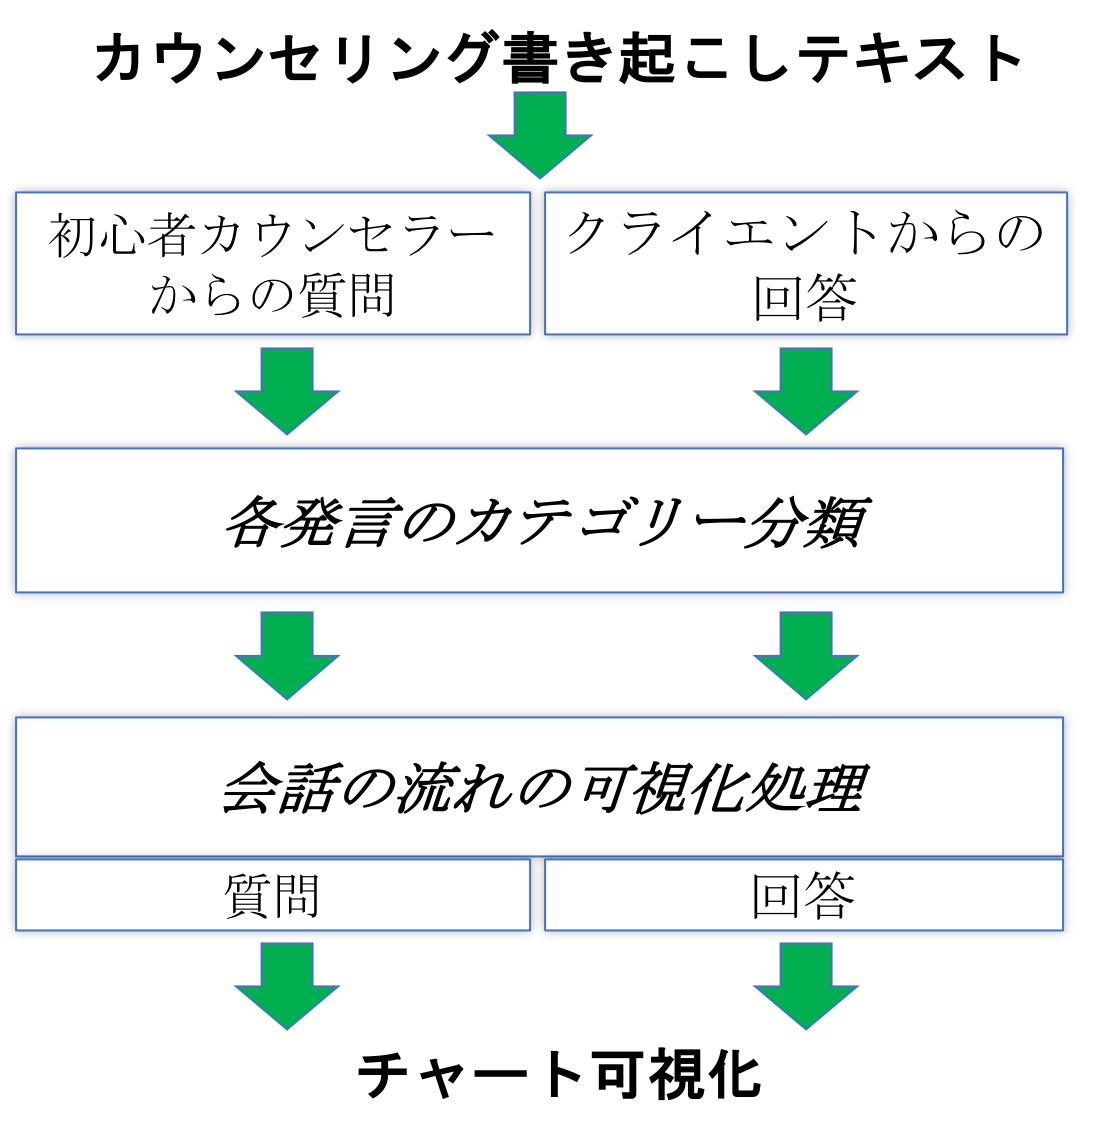
\includegraphics[width=\linewidth]{4_2.png}
   \end{center}
   \caption{提案システムの構成}
   \label{fig:4_2}
 \end{figure}

\begin{figure}
   \begin{center}
     % 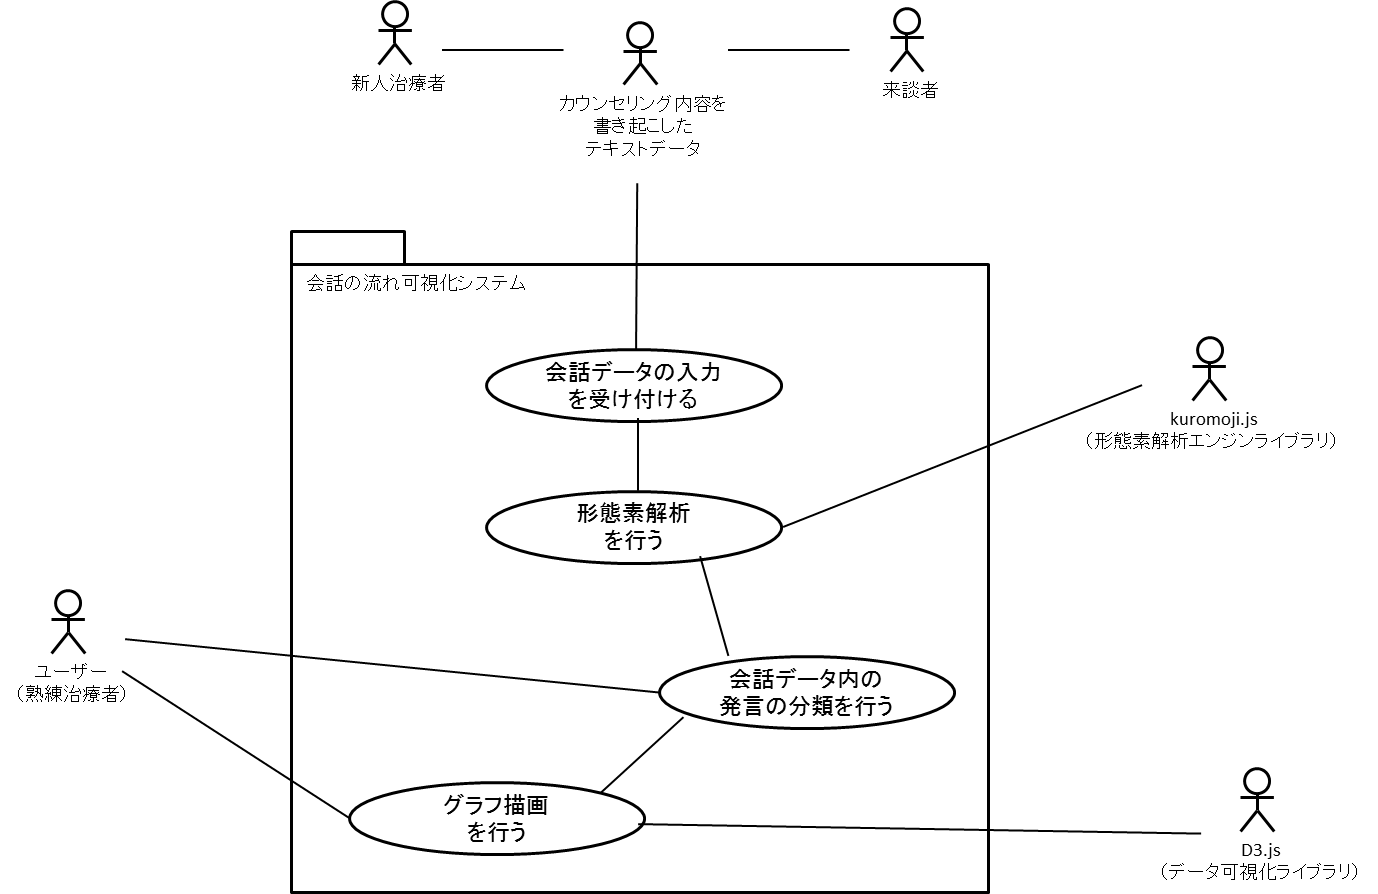
\includegraphics[width=\linewidth]{use_case_diagram.png}
   \end{center}
   \caption{提案システムのユースケース図}
   \label{fig:use_case_diagram}
 \end{figure}


まず,グラフ描画前のテキストデータ処理について述べる.アクティビティ図を図
%\ref{fig:activity}
に示す.アクティビティ図とはフローチャートに似た図で,いわゆるビジネスロジックにおける手続き的な流れやプログラムの制御フローを表すUMLの図である.
\begin{figure}
   \begin{center}
     %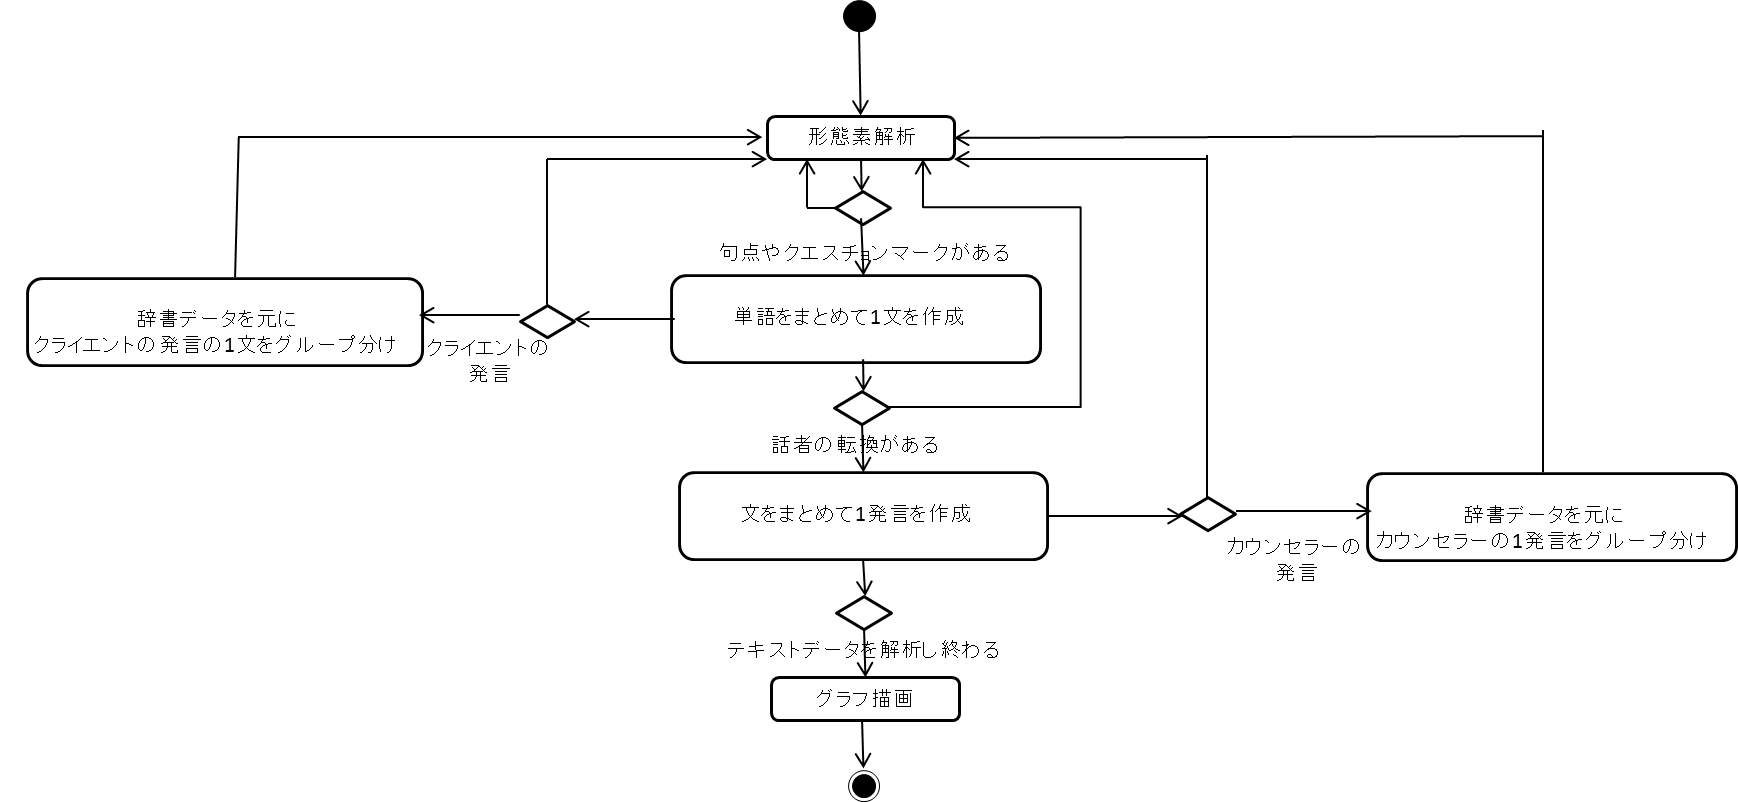
\includegraphics[width=\linewidth]{activity.png}
   \end{center}
   \caption{テキストデータ処理のアクティビティ図}
   \label{fig:activity}
\end{figure}


初めに,ブラウザ上で各テキストの会話データを読み込んで,テキストを単語ごとに区切る形態素解析を行う.会話データ読み込み前の本提案システムスクリーンショットを図
%\ref{fig:yomikomimae2}
に示す.
 \begin{figure}
   \begin{center}
     %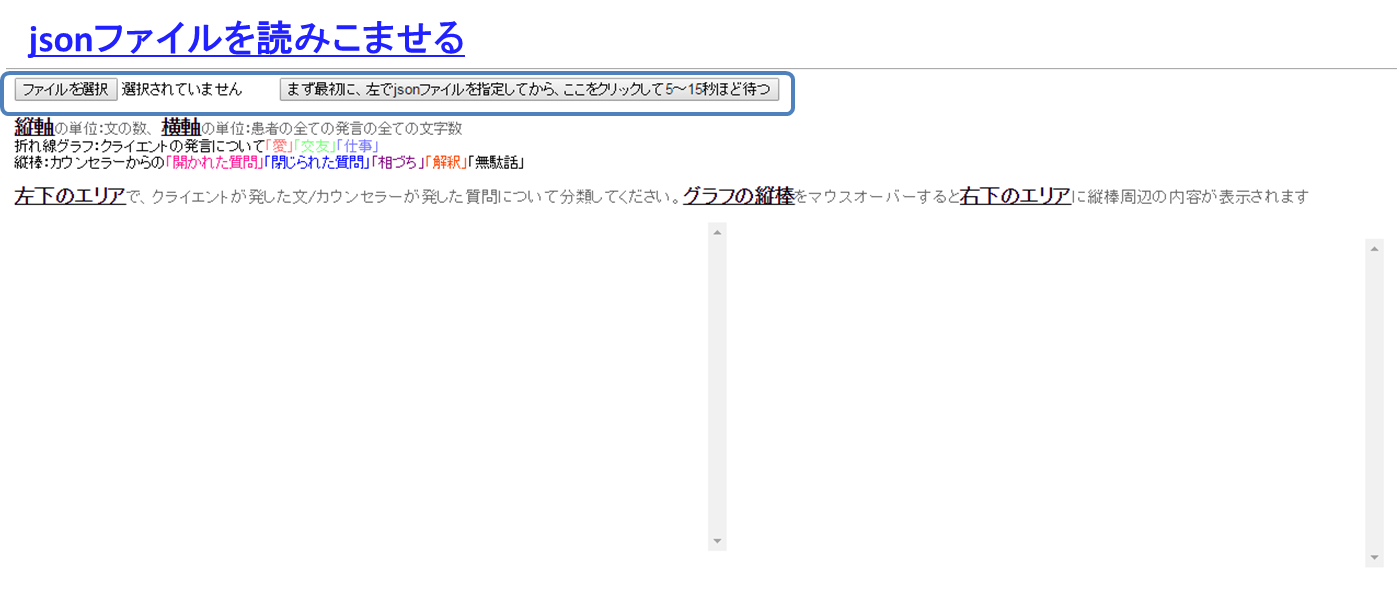
\includegraphics[width=\linewidth]{yomikomimae2.png}
   \end{center}
   \caption{会話データ読み込み前のシステムスクリーンショット}
   \label{fig:yomikomimae2}
 \end{figure}
形態素解析サブシステムには,JavaScript言語の形態素解析ライブラリであるkuromoji.js\cite{kuromojijs}を使用した.kuromoji.jsは,Javaで実装されたオープンソースの日本語形態素解析エンジンKuromoji
%\cite{kuromoji}
を,JavaScriptに移植したものである.

\subsection{1文や1発言の作成と分類}
形態素解析された単語群から,句点やクエスチョンマークを終点と定義して1文ずつのテーブルをつくる.さらに,話者の切り替わりを全角コロンで定義し,全角コロンと全角コロンの間の文のグループを1発言と定義し,発言単位でテーブルをつくる.「クライエントの発言においてこれを含む文はこのグループに属するだろう」という単語を,「愛」「仕事」「交友」ごとに指定しておき,発言データの文を構成する単語が指定された単語と一致する場合,この情報を図
%\ref{fig:4_2}
の発言データ分類サブシステムに引き渡し,発言データ分類の初期設定値を計算する.
%この初期選択において,今回は簡単化のため,複数のグループの可能性をもつ1文に対しては,「愛」の可能性があれば「愛」に,それ以外は「仕事」に分類するようにした.



.






前節で述べた要件抽出にもとづいて、我々は会話の流れ可視化システムの開発を行った。本節では、会話の流れ可視化システムの、可視化する前の処理の部分について説明を行う。



  臨床的観点からは、三つのカテゴリーに人間の問題を分類するために極めて有効であると考えられる。上記分類方法から、我々は次のサブセクションで提案されたシステム、設計および実装するための要件のextrbehaviorを説明する。


  このセクションでは、提案システムの設計と実装について説明する。図3は、カウンセリングでの会話の流れの可視化システムの処理手順を示している。会話の流れの可視化は)1つのカウンセリングセッションでの会話の内容を示している。このシステムでは、可視化の前処理として、カウンセリングにおける会話のテキストデータのカテゴリ分類が実行される。


まず、提案システムは、ブラウザ上で各テキストの会話データを読み、言葉にテキストを分離するために形態素解析を行いる。使用されたJavaScript言語の形態素解析ライブラリである形態素解析サブシステム、kuromoji.js [13]のために。 kuromoji.jsはJavaScriptに移植されたJava Kuromoji [14]に実装オープンソース日本語形態素解析エンジンである。

  次に、これらの文章は、このシステムに登録カテゴリーと文の各単語に対応するキーワードとのマッチングにより、各カテゴリに分類されている。しかし、このカテゴリの分類方法ではカウンセラーとクライアントによって各発話のテキストデータに適用し、分類結果の精度は、システムに登録されている単語辞書に依存し、分類のための正解率は非常に低いである。そのため、専門家のカウンセラーは、現在のシステムでは、最初の分類結果を確認し、手動で誤った分類結果を修正する必要があり、作業負担が大きい。クライアントのそれとは違って、私はセラピストの発話の分類は、文単位が、話し手ターン単位での分類ではないというコメントを得た。


  従って、このシステムでは、担当者やカウンセラーからの1つのコメントは話者の変更によって判断される。カウンセラーが話し終えるとクリニックが話すと、治療が話し始めるまで話者が、話し始めるまで、言い換えれば、話者の1から1件のコメントである。また、ずつutterancはe  、 カウンセラー話者が話し、またはカウンセラーが話し終わるまでカウンセラーが、話を引き裂く起動し、情報提供者が話し始める終了時からである。

  このシステムでは、クライアントの発話は、それぞれの文は、アドラー心理学に基づいて、タスクエリア「仕事」、「友情」と「愛と家族」に相当する。図4は、表.2のようにカウンセラーの質問の自動分類方法の流れを示し、表2に示すように、他の手で、初心者カウンセラーによって発声は5つのカテゴリに分類されている。まず、「いつ」、「どこで」、「何を」として、「5W1H」を示すinterrogatives、との声明を分類し、その上の「オープン質問」など。次に、残りの発話のうち、5つの以下の単語を有するものは、「フィードバック」として分類される。さらに、残りの発話のうち、「KA」日本の最終的な封入粒子を含む発話が「閉質問」として分類される。限り過去、「解釈は」日本最後のエンディングの粒子「NE」と「アイドルの話」を含むもののために含まれているとして分類されていなかったものの中に日本人が含まれないものを除外することである。


\subsection{クライエントの回答に関する分類} %%%%%%%%%%%%%%%%%%%%%%%%%%



クライエントの発言に関する分類に関しては,1発言単位ではなく1文単位で「愛」「交友」「仕事」を分類するように変更することが求められる.
たとえば,「うちの夫は仕事にいくのを嫌がって,毎朝起きてこないんである.
それを見ているだけで腹が立つんである.自分の同僚が同じように仕事に行きたが
らなくて朝起きなかったという話を聞いても,さほど腹は立ちないが,夫がそ
うなるのは絶対に許せない」という文章について,専門家は次の通りに分類する.第1文は愛の課題,第2文は仕事の課題,第3文は愛の課題に分類する.

原文から,カウンセラーからクライエントへの質問事項の分類の指標として,クライエントの発言をうながしてクライエント自身も気づいていなかったことを認知させるのが大事であるので,それぞれの発言量の可視化の実装を盛り込むべきであるというコメントを得た.ここから得られる要件は,クライエントの発言の分量に応じて,それをはさむカウンセラーの発言の縦棒をグラフ上で変えることであると考えた.

したがって、クライエントの発言に関する分類に関して、図〜〜に示すアルゴリズムで分類を行った。まず--

発話データの分類後、クライアントによる発声のための初心者カウンセラーと「仕事」、「友情」と「愛と家族」に関連した文のカテゴリグループのための時系列での分配変化による質問の形式は、同じ時代に可視化した。

\subsection{カウンセラーの質問に関する分類} %%%%%%%%%%%%%%%%%%%%%%%%

カウンセラーの1発言についても,クライエントの発言の1文ごとの分類と同様に,関連する単語をあらかじめ指定しておき,必要情報を
%\ref{fig:4_2}
の発言データ分類サブシステムに引き渡し,発言データ分類の初期設定値を計算する.

ここで会話データを入力した後のカウンセラーの初期分類状態の分類方法について説明する.今回の実際の会話データ15個のうち,カウンセラーの発言数は398発言あったが,本システム要件の質問分類の「相槌」に含まれるべき短文に「そうであるか」というフレーズが41箇所あった.富士通株式会社は質問文判定について特許
\cite{tokkyo}
を取得しているが,富士通株式会社の特許技術において行われている「(る)か」という文の終わり方だけで質問判定を行うだけでは,「そうであるか」というフレーズも自動的に「相槌」ではなく「閉じられた質問(Closed-ended Question)」に分類してしまうので不適当である.

カウンセラーの発言の分類について,まずカウンセラーの発言も,次章で述べる初期分類は適当ではないことがあるので,クライエントからの返答だけでなく,カウンセラーの質問区分けも手動で修正したいというコメントを得た.

また,カウンセラーの発言について,「開かれた質問(Open-ended Question)」「閉じられた質問(Closed-ended Question)」だけでなく,「解釈」「相槌」「世間話」という分類を追加してほしいというコメントを得た.

クライエントの発言に関する分類とは異なり,カウンセラーの発言に関する分類は1文単位ではなく1発言単位での分類でよいというコメントを得た.

したがって、クライエントの発言に関する分類に関して、図〜〜に示すアルゴリズムで分類を行った。まず〜〜




質問内容は,前章の要件通り 5 種類に分類され,後述する縦棒アイコンの色の割り当ては次の通りである.赤色は5W1H「いつ」「どこで」「誰が」「何を」「どのように」「どうした」などで問われるような「開かれた質問(Open-ended Question)」,青色はYes/Noで答えられる,あるいは一言だけで簡単答えられるような「閉じられた質問(Closed-ended Question)」,紫は「相槌」,オレンジはクライエントの問題をカウンセラーがどう「解釈」しているかの確認,黒は「世間話」を表現している.第1章で述べた通り,クライエントが何に問題意識を感じているかをカウンセリングで引き出すには,カウンセラーは「閉じられた質問(Closed-ended Question)」よりも「開かれた質問(Open-ended Question)」をしたほうがよいとされている

我々2)3)が開発したカウンセリングにおける会話の流れ可視化システムの構成をFig.1に示す.まず会話データ入力サブシステムでカウンセリングの書き起こしテキストデータを入力し,形態素解析サブシステムに引き渡す.
形態素解析サブシステムでは,カウンセラーの1発言についても,クライエントの発言の分類と同様に,関連する単語をあらかじめ指定しておき,必要情報をFig.1の発言データ分類サブシステムに引き渡し,発言データ分類の初期設定値を計算する.本システムにおける,会話データを入力した後のカウンセラーの初期分類状態の分類方法をFig.2に示す.

はじめに,「いつ」「どこ」「何」などの5W1Hを示す疑問詞を含む発言を「開かれた質問」に分類する.次に,残りの発言から単語数が5個以下のものを「相槌」に分類する.さらに残りの発言で終助詞「か」を含む発言を「閉じられた質問」に分類する.これまでの3パターンに分類されなかったものは「解釈」か「世間話」に分類されるが,
終助詞の「ね」を含むものを「解釈」,含まないものを「世間話」とした.
一方,クライエントの発言の各1 文の分類方法として,ヨーガセラピーが基本としているアドラー心理学の3つのライフタスク7)(「愛」「仕事」「交友」)分類カテゴリとして用いることにした.
次に,会話データを発言データ可視化サブシステムに受け渡し,カウンセラーからの質問の分類結果と,クライアントの発言のカテゴリ分類結果を併せて,時間経過に沿った分布変化としてグラフによる可視化表示を行う.


\section{可視化結果}

前節では、会話の流れ可視化システムの可視化前の処理の部分の実装について説明を行った。本節では、その前処理後の可視化の処理の部分について説明を行う。


%%可視化結果をゴリゴリ説明

図 に時系列人間関係チャートの画像を示している。下

%のスライダーを動かすことによって、我々はどのような文を時系列に沿ってどのような文に、例えば、人間関係からチャートを表示した。また、図2に示すように、それが可能な、対応する動詞の文章を表示することによって、我々は、矢印は、図手段として、元のどのテキストを知ることができる。

我々は、可視化のためにD3.js\cite{vand3}を用いた。D3.jsはウェブブラウザ上で動的なコンテンツを可視化するためのJavaScriptのライブラリであり、ニューヨーク・タイムズ紙サイト内のグラフ描画などに用いられている。



本システムにおける,会話データを入力した後のカウンセラーの初期分類状態の分類方法を簡単に図
% \ref{fig:5_2}
に示す.
% \begin{figure}
% %\begin{landscape}
%    \begin{center}
%      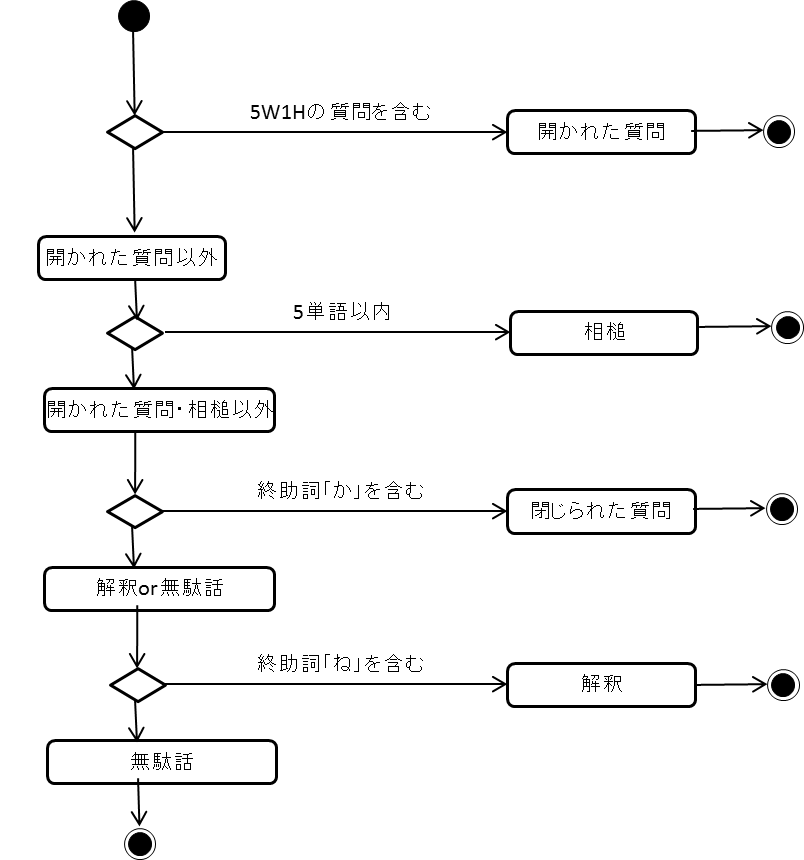
\includegraphics[width=\linewidth]{5_2.png}
%    \end{center}
%    \caption{カウンセラー発言初期分類方法}
%    \label{fig:5_2}
% %\end{landscape}
%  \end{figure}
まず「いつ」「どこ」「何」などのいわゆる5W1Hを示す疑問詞をもつ発言を「開かれた質問(Open-ended Question)」に分類する.次に残りの発言のうち,単語数が5個以下のものを「相槌」に分類する.さらに残りの発言のうち終助詞「か」を含む発言を「閉じられた質問(Closed-ended Question)」に分類する.今までの3つに分類されなかったものは「解釈」か「世間話」に分類されるわけだが,終助詞の「ね」を含むものを「解釈」,含まないものを「世間話」とした.

\subsection{グラフ描画}
以上がグラフ描画前のテキストデータ処理である.その後,カウンセラーからの質問形態と, 「愛」「仕事」「交友」の文のグループの時間経過に沿った分布変化を可視化する.グラフ描画の際に,会話データを発言データ可視化サブシステムに受け渡す.このサブシステムでは,データ可視化ライブラリD3.js
%\cite{bostock2012d3}
を使用した.模擬会話データを入力した際の出力結果を図
% \ref{fig:6_1}
に示す.また模擬会話データの原文と,模擬会話データ時の初期自動分類結果を表
% \ref{table:book1}
に示す.
% \begin{figure}
%    \begin{center}
%      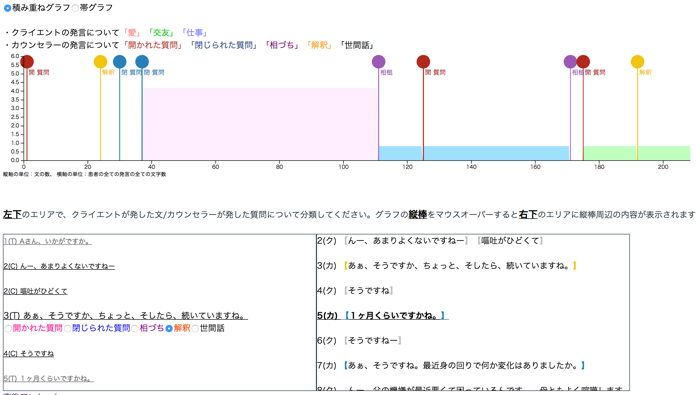
\includegraphics[width=\linewidth]{6_1.png}
%    \end{center}
%    \caption{模擬会話データでのシステム出力結果}
%    \label{fig:6_1}
%  \end{figure}
%
% \begin{table}
%    \caption{模擬会話データでの初期表示用自動分類結果}
%    \label{table:book1}
%    \begin{center}
%      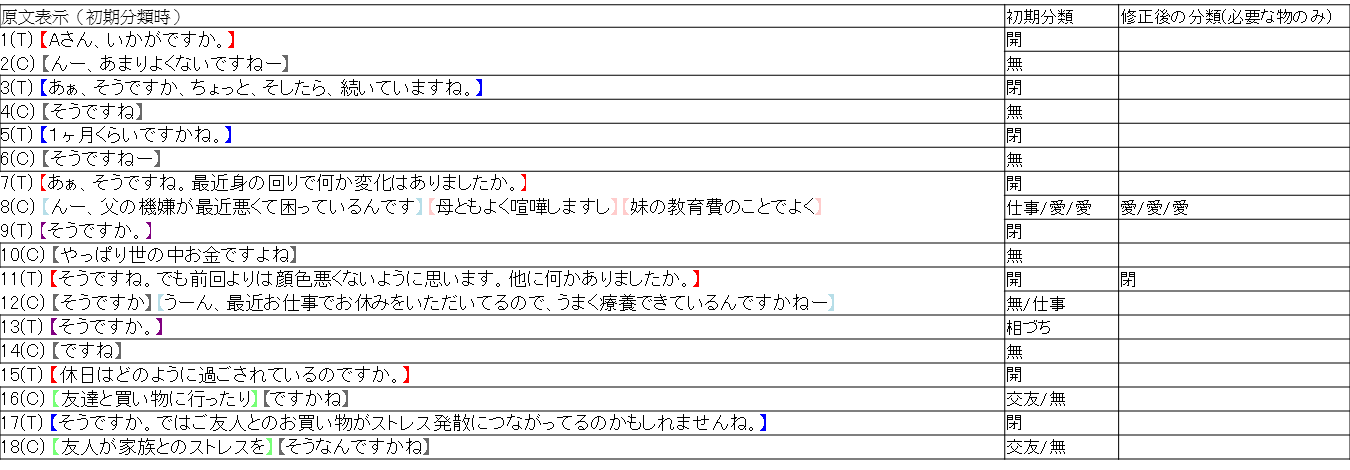
\includegraphics[width=\linewidth]{book1.png}
%    \end{center}
%  \end{table}

\subsection{クライエント発言ビュー}
次に〜〜について用いる、クライエント発言ビューについて説明する。
図
%\ref{fig:6_1}
において,まず積み重ね折れ線グラフはクライエントの1回の発言の中での,アドラー心理学の各カテゴリの分布を可視化している.ただし1回の発言は,話者の交代を発言の区切れ目とする.この積み重ね折れ線グラフにおいて薄い水色は「仕事関係」,ピンク色は「愛(恋愛・愛関係)」,薄い緑色は「交友(友人関係)」に密接に関係する単語を含む文の分布を表している.

横軸は時間軸を表現している.ただし対象データである書き起こしテキストデータからは実際の経過秒数は読み取れないので,読み込ませたデータ内におけるクライエントの発言量の累計の文字数を横軸,つまり時間軸とした.後述するカウンセラーの質問を表現する縦棒はこの時間軸にそって出現する.カウンセラーとクライエントの発言の入れ替わりがわかりやすいように,積み重ね折れ線グラフがクライエントの発言のグループ分布をちょうど表しているのは便宜上発言部分の中央部分になっている.

縦軸は発言中の1文の数のうち,どのグループに何文入っているかという文の数を表している.

%ここで会話データを入力した後のクライエントの発言の各1文の初期分類状態の分類方法について説明する.
%まず,あらかじめこちらで
%次に,各単語群を含むクライエントの発言の1文をグループ分けをしていった.




\subsection{カウンセラー発言ビュー}

Ericら\cite{taskdriven}
は,トピックモデリングによって分けたトピックの時間分布を上下の非対称積み重ね折れ線グラフによって可視化した.一方本研究では,カウンセラーとクライエントの会話において,クライエントは文ごとに,カウンセラーは発言ごとに描画を行いたい,かつ選択肢表示のためにグラフを省スペースしたいという観点から,カウンセラーの発言を横軸より下に折れ線グラフとして描画するのではなく,クライエントの発言のグループ分布を示す積み重ね折れ線グラフに重ねて縦棒として表示するようにした.こうすることによって,クライエントとカウンセラーの発言が交互に描画されるので,クライエントとカウンセラーの発言の関連性がわかりやすくなった.積み重ね折れ線グラフに重なっている縦棒は,カウンセラーの質問内容の形態を示す.


\subsection{発言分類手動修正機能}
積み重ね折れ線グラフが描画された後に,グラフ左下のラジオボタンエリアにて,クライアントの発言の各1文およびカウンセラーの各1発言において,分類を変えると即時にグラフ描画に変更が適用されるようにした.
%本ラジオボタンエリアがみたした要件については,付録にて記述する.

%\section{要件抽出}



%\section{開発}

%%修論からパクってくる



\subsection{ケーススタディ}

前節までで、本システムの前処理手順および可視化手法と可視化結果について述べた。本節では本システムにもとづいたユースケースについて述べる。

\section{ユーザー評価実験と考察}

前節までは、会話の流れ可視化システムの開発およびケーススタディについて説明を行った。本節では、会話の流れ可視化システムを用いて「」という仮説を検証するために行ったユーザ評価の目的・手法・結果・考察についてのべる。カウンセラー習熟度評価支援システムは、主に、

%%ユーザエバリュエーションをゴリゴリ説明




  専門カウンセラーが、彼は「私はBが私の意志に従うことをしたい」という考えが消えていることが分かったと述べた。

自己閉じタスクが増加した。認知の補正の進行は、することができた 量変更することによって確認 矢印の(複数カウンセリングの全体図)をし、元のテキスト表示で品質を確認。 我々は、我々の提案文字チャートの可視化は、カウンセラーは見つけることができることを検討してください のいくつかの種類がことを 、クライアントの 認知の修正作られた。

\subsection{シグマ値法}
多数の意見項目などを多変量解析で分析する際に、態度を測るものさしであるカテゴリー尺度は、本来は順序尺度なので、間隔尺度に換算して重み付ける必要がある。しかし通常は、回答ガテゴリーのコード番号を間隔尺度の得点として簡便に用いている。

通常の例の場合に対して、心理学では、カテゴリーの順序尺度を間隔尺度に換算する方法を持っている。その一つにシグマ値法(系列カテゴリー法ともいう)が存在する。シグマ値法は、意見項目の各カテゴリーに対する一連の回答率を、標準正規分布の面積と考え、面積に対応する縦座標と面積の比という間隔尺度に置き換える方法である。

標準正規分布は、元のデータを0、標準偏差1.0に換算したデータのことである。シグマ値法においては、回答カテゴリーの回答率を標準正規分布の面積と考えて、面積に対応する縦座標の比に置き換えることによって、順序尺度を間隔尺度に置き換えることが出来ている。

シグマ値法は以下の手順に従って算出される。
\begin{enumerate}
 \item 各カテゴリーの順番を下位のものから上位のものに整列させる
 \item 格カテゴリーへの度数から比率を計算する
 \item 各カテゴリーの累積の比率を算出して、下限値から上限値までを計算する。
 \item 各カテゴリーの累積の比率の最小値と最大値を標準正規分布の縦座標に置き換える
 \item シグマ値を計算する
 \item カテゴリー得点の計算を行う。
\end{enumerate}

以上のシグマ値法で換算した値を用いて、多変量解析をおこなうことによって、「悪いが1点、やや悪いが2点、……」のようなカテゴリー得点をカテゴリーの数字で代替する通例の手法よりも明快な解析結果が得られると言われている。

ガウスの誤差関数
\begin{equation}
  erf(x) = \frac{2}{\sqrt{\pi}}\int_0^x e^{-t^2} dt
\end{equation}
を用いると、標準正規分布の累積分布関数F(x)は
\begin{equation}
  F(x) = \frac{1}{2}(1+erf\frac{x}{\sqrt{2}})
\end{equation}
で表される。この逆関数\begin{equation}F^{-1}(x)\end{equation}を用いて、標準正規曲線の面積に対応する標準得点Z(p)は

%Z(p)=-F-1(1-p)

\begin{equation}
  Z(p) = -F^{-1}(1-p)
\end{equation}

でである。標準得点Zに対応する縦座標yは、標準正規曲線の確率密度を求める式によって表され、
\begin{equation}
y(Z)=\frac{1}{\sqrt{2\pi}}exp(-\frac{Z^2}{2})
\end{equation}

となる。






\subsection{形状比較に関する評価と考察}
上辻の卒論で取り扱った形状との比較を行った。

前章で述べた会話の流れの可視化システムを,3名の熟練のカウンセラーに評価者として実際に使用してもらうことで,システム評価を行った.
熟練のカウンセラーの平均年齢は55歳,平均臨床歴は29年であった.

\subsubsection{6段階評価のアンケート}



まず評価者は,積み重ねグラフ,帯グラフそれぞれについて,あらかじめ表示されている可視化結果に対して,時系列に沿ってマウスカーソルを合わせることで,カウンセリングの流れを一通り確認する.その後,6段階評価によるアンケート質問に回答を行う.6段階評価のアンケートの質問項目,および各質問に対する選択肢とその配点をTable 1に示す.Table 1の各質問項目は,積み重ねグラフ,帯グラフそれぞれに対して行った.積み重ねグラフ,帯グラフについて,各質問項目に対する6段階評価の平均値の結果をFig.5に示す.Fig.5 の結果より,全ての項目において,積み重ねグラフより帯グラフの方が優れていることがわかった.

%%有意差、相関関係

\subsubsection{自由記述のアンケート}

さらに本評価では,以下の(1)~(5)に記す自由記述の 質問を行った.

(1)	帯グラフを見て,カウンセラーに対してどのような指導ができるでしょうか
(2)	グラフについて,その他全体的に何かご意見が  あれば,ご回答ください
(3)	このシステム全体を用いて,カウンセラーに対して指導できそうなことがあれば,ご回答ください
(4)	原文表示機能について何かご意見があれば,ご回答ください
(5)	このシステムについて,何か他に欲しい機能が  あれば,ご回答ください

質問(1)に対して

  一回のカウンセリング全体を俯瞰し大まかな カウンセリングの流れを指導
  クライエントとカウンセラーが時系列で対比 しながら見ることができるので,一回の面接での流れ,例えば,前半はクライエントに多く喋ってもらっていたのが,後半ではカウンセラーが喋っていたとか,解釈の時に発言量が多いとかが指導できるように思いた

といった回答が得られた.これより,全体を俯瞰して発言量の分布の変化を基に初心者カウンセラーに対して,様々な指摘を行えることが考えられる.
質問(2)に対しては「帯グラフで,それぞれの発言内容の語数や時間が表示されれば,さらに便利かなと思いた」という回答が得られた.
質問(3)に対しては

  カウンセラーの発言のチェックとクライエントの関心に関心を向けているかのチェック」「一回のカウンセリングでカウンセラーとクライアントがどのような作業を協力して行っているのか理解を深めること,カウンセリングが成立するためにはカウンセラーとクライアントの間で相談的人間関係が構築できていることが前提となることを理解するのに役立つ
  カウンセリングがこのように可視化されることだけでも,とても有意義だ
  この結果をもとに,カウンセリングを再構築するための材料としても使える

といった回答が得られた.
質問(4)に対しては「カウンセラー,クライアントがどこでどんな発言をしているのか確認するのに役に立つと思いた」という回答が得られた.
以上の結果から,積み重ねグラフよりも帯グラフの方が,初心者カウンセラー指導に優れていると結論づけられる.また全体として,本システムが初心者カウンセラーに対する指導を行うために,会話の流れが適切に可視化されていることが,複数名の熟練のカウンセラーからの回答によって結論づけられると考える.
 質問(5)に対しては

  カウンセラー,クライアントの発言を音声で確認できる機能,カウンセリング中のクライアントの身体の動きの変化(カウンセリング開始から本題にはいるまで〈相談的人間関係構築がなされているかどうか確認のため〉また特にカウンセラーが解釈投与した直後のクライアントの身体の動き〈解釈投与に対してクライアントがどのような認識反射をおこなっているのかを確認するため〉)についても記されていると便利だと思いる
  複数の内容が入った文について,うまく分類できればもっと便利
  内容分類項目のアレンジ機能(追加,修正)


%%コメントでページ数稼げる

といった回答が得られた.
以上の回答から,本システムのユーザービリティの 改善や機能追加についてさらなる検討を行う必要があり,今後の課題とされる.

\subsection{原文を読むこととの比較評価と考察}

%%コメントでゴリゴリ稼げる



前サブセクションでは、上辻らが2015年に発表した積み重ね折れ線チャートよりも、本稿で提案した本システムの帯グラフの方が、初心者カウンセラーに対する指導を行うためにより適切な可視化方法であることが分かった。この前サブセクションで述べたユーザー評価からわかったことを元に、実際のカウンセリング内容の原文を用いて、実際のカウンセラー内での事例検討会に近いスタイルフォーマットの原文のみを読んでの初心者カウンセラー指導と、本稿で提案した帯グラフを用いた初心者カウンセラー習熟度評価支援システムを用いての初心者カウンセラー指導との比較実験について、本サブセクションにて述べる。

で述べた会話の流れの可視化システムを,3名の熟練のカウンセラーに評価者として実際に使用してもらうことで,システム評価を行った.熟練のカウンセラーの平均年齢は55歳,平均臨床歴は29年であった.

\subsubsection{6段階評価のアンケート}

まず評価者は,積み重ねグラフ,帯グラフそれぞれについて,あらかじめ表示されている可視化結果に対して,時系列に沿ってマウスカーソルを合わせることで,カウンセリングの流れを一通り確認する.その後,6段階評価によるアンケート質問に回答を行う.6段階評価のアンケートの質問項目,および各質問に対する選択肢とその配点をTable 1に示す.Table 1の各質問項目は,積み重ねグラフ,帯グラフそれぞれに対して行った.積み重ねグラフ,帯グラフについて,各質問項目に対する6段階評価の平均値の結果をFig.5に示す.Fig.5 の結果より,全ての項目において,積み重ねグラフより帯グラフの方が優れていることがわかった.

%%有意差、相関関係
\subsubsection{自由記述のアンケート}


さらに本評価では,以下の(1)~(5)に記す自由記述の質問を行った.



\begin{enumerate}
 \item 帯グラフを見て,カウンセラーに対してどのような指導ができるでしょうか
 \item グラフについて,その他全体的に何かご意見が  あれば,ご回答ください
 \item このシステム全体を用いて,カウンセラーに対して指導できそうなことがあれば,ご回答ください
 \item 原文表示機能について何かご意見があれば,ご回答ください
 \item このシステムについて,何か他に欲しい機能があれば,ご回答ください
\end{enumerate}




%%コメントでページ数稼げる





%%%%%%%%%%%%%%%%%%%%%%%%%%%%%%%%%%%%%%%%%%%%%%%%%%%%%%%%%%%%%  4章
%%認知の修正
\chapter{クライエントの認知の修正評価支援システム}
	\section{目的}


\section{要件抽出}

クライアントの認知補正の分析は、何らかの形でのように述べた行動クライアントのカテゴリを使用 図。2 動作は、クライアントの周りの人々が行っていたものが挙げられる。 鎌田によると\cite{kamata2002}、 カウンセラーの行動や感情を重要な役割は、クライアントが自己決意と自己責任を取ると不当に他人に介入することなく、他者との協力関係を形成することができるようにクライアントを奨励することである。だから、不当に他人の行動や感情に介入することなく、クライアント自身の行動や感情を見つけることが重要である。

  カウンセリングで、「自分の行動を変えるのではなく、相手の行動を変えることに興味がある人は、認知を修正するに進んでいる」と言われている。ときに、クライアントの答え「クライアント自身の行動」ではなく答えるクライアントの認識の修正が進んでいると言われて、 『クライアントの周りの人々の行動を。』

  我々は、または「クライアント自身の行動」「クライアントの周りの人の行動」のデータを視覚化することにより、クライアントの知覚の状態を確認できることを考えた。一方、我々は年代順に会話内容をテキストで行動の対象と述語を可視化することにより、上記のニーズを満たすことができると考えた。このようなニーズに応えて、我々は行動の対象とオブジェクトの情報を含む人間関係チャートの時系列を視覚化してきた。



\section{前処理の開発}

  このセクションでは、人間関係を生成するためには、直列に沿った、チャート、我々は時間データと行動データを抽出する方法、対象データを説明し、テキストデータ内のオブジェクトデータ。 図5は、前手順の流れを示している.

  このサブセクションでは、文章中の文字を抽出する方法について説明して。カウンセリング会話書き起こしテキストデータをKNPに入力されたときに、このシステムの入力は、KNP [15](依存アナライザ)の出力結果である。次に、ある言葉(文字候補)「カテゴリ:人は」抽出した。その後、元の文は、形態学的日本語形態素解析器JUMAN\cite{juman}によって分析される。 JUMANは、形態素解析時に、独自の辞書によって、日本の各単語を分類する。したがって、JUMANにより「人」のカテゴリに分類された単語を抽出することにより、我々は、文章中の文字を抽出した。

  また、我々は動詞のリストを得た。我々は対象を取得または各動詞の対象とすることができるように次に、我々は、それぞれの動詞の周りの依存関係を把握した。
  その後、我々は対象とカウンセリング会話テキストが持つオブジェクトの同じペアを持っているどのように多くの動詞を数える。我々は、円や矢印の意味の動詞の数によって、図1のグラフに円や矢印のストローク幅を追加する。


  \subsection{係り受け解析}


「構文解析(こうぶんかいせき、syntactic analysis あるいは parse)とは、文章、具体的にはマークアップなどの注記の入っていないベタの文字列を、自然言語であれば形態素に切分け、さらにその間の関連(修飾-被修飾など)といったような、統語論的(構文論的)な関係を図式化するなどして明確にする(解析する)手続きである。自然言語については自然言語処理における要点のひとつであり、プログラミング言語など形式言語の場合は、形式文法に従い構文木を得る。構文解析を行う機構を構文解析器(parser)と呼ぶ。」
  KNP


  \subsection{登場人物と動詞の抽出}


  \subsection{動詞の主語と目的語の抽出}

\subsubsection{動詞の主語の抽出}
\subsubsection{動詞の目的語の抽出}


%%%%%$ 認知の修正可視化結果

\section{可視化}

この章で、我々は我々の提案システムの可視化結果を説明する。この提案されたシステムにおける会話の流れの可視化結果の図6と3例を示する。可視化結果は、3つの項目から構成されている。我々は、可視化のためにD3.js [17]を使用していた。%それが書かれた書き起こし産物に基づきる。



\subsection{人間関係図}

田中らは無向グラフによる可視化であったが、

  Fig.1 shows the image of the time series human relationship chart. By moving the lower slider, we displayed the human relations chart from, for example, what sentence to what sentence along the time series. Moreover, as shown in Fig.2, by making it possible to display the sentence of the corresponding verb, we can know which original text the arrow means as Fig. 7. We used D3.js[17] for the visualization.


Fig.1 An example of the time-series visualization of character chart with behavior arrow from the dependency analysis of the text data. The arrows show behavior. Circle shows behavior that means (1) or (3) of chart Gray arrow means (4) or (5). Red arrow means (2). Slider selects the visualized area of the input text. If we click a circle or a arrow, the original texts including verbs which the circle or the arrow appear at the left side of the screen as Fig.7.

Fig. 7 Full view of our character chart visualization. If we click a circle or a arrow, the original texts including verbs which the circle or the arrow appear at the left side of the screen

\subsubsection{会話文中の登場人物の内的感情や一人で完結した行動を表す円形}

カウンセリングの会話内に登場する人物について、その会話中でその人物が起こし、その人物自身で閉じた行動の数:円の大きさクライエント自身であれば円はピンク、それ以外は水色


\subsubsection{会話文中の登場人物が別の登場人物に対して行った行動を表す矢印}

矢印は「誰か」から「誰か」への行動の発生を表している。
矢印の直線の太さで、その行動の数を表現している。
前節でカウントした、「主語・目的語の組み合わせが同じ動詞」を1つの「矢印」にまとめ、その「動詞」の数を「矢印」の太さで表現している。

人物から別の人物へ起こった行動の数:矢印の太さで表されている。
「クライエント」から「周囲の人」へのポジティブな行動:(「ネガティブだが、もしもの話」の場合を含む)
→赤の矢印
「クライエント」から「周囲の人」へのネガティブな行動:(「ポジティブだが、もしもの話」の場合を含む)
→青の矢印
「周囲の人」から誰かへのポジティブな行動:(「ネガティブだが、もしもの話」の場合を含む)
→グレーの矢印
「周囲の人」から誰かへのネガティブな行動:(「ポジティブだが、もしもの話」の場合を含む)
→緑の矢印



\subsection{スライドバー}

カウンセリングの会話の原文のうち、200文分を上記グラフにて可視化しておりる。初期表示では0文目〜200文目についての グラフを表示している。

青丸にマウスカーソルを合わせると、いま何文目から何文目までについての可視化を行っているか、吹き出しで表示される。
青丸を動かすことで、可視化する会話文の範囲を変えることができる。


\subsection{原文表示機能}

グラフの登場人物の円をクリックすると、「その登場人物が登場するカウンセリングの原文箇所」が、画面右側に表示される。
グラフの矢印をクリックすると、右側に「その矢印に該当する行動を示すカウンセリングの原文箇所」が、画面右側に表示される。描画に10秒ほど時間がかかる場合がある
原文表示で下線が引かれている場所に、そのクリックした矢印に該当する動詞が含まれている




\section{ケーススタディと考察}

  The expert counselor said that he found out that the idea "I want B to follow my will" disappeared
and self-closed task increased. Progress of correction of cognition could be confirmed by changing the quantity of arrows (Overall view of multiple counseling) and confirming the quality in original text display. We consider that our proposed character chart visualization helps counselors find out that some kind of client's cognitive fixes were made.

  図1 カウンセリング1
  図2 カウンセリング2

  「色付きの方がネガティブとポジティブについてわかりやすい」

・矢印の分類の信憑性の問題
は、テキスト分析の問題なので、future work にせざるを得ない(会話の流れと同様)

%%%結論
\chapter{結論}

本章では、本稿における結論、および、本稿で述べた内容の将来性について述べる。

\section{結論}

本研究では,時間軸に沿った可視化によって,クライエントとカウンセラーの会話の流れを可視化するWebシステムを開発した.熟練のカウンセラーから初心者へのカウンセリング指導において,どのような質問を初心者カウンセラーがクライエントに投げかけるかによって,初心者カウンセラーがクライエントからどのような「対人関係上の問題」に関する回答を引き出せたかが重要である.それが一目見てわかるようになったことが,本システムにて実現されたことであると考える.特にこの実現について寄与するものであると筆者が考えるのは,縦棒同士の間隔が等間隔であるグラフデザインよりも,縦棒同士の間隔のクライエントの発言の文字数に比例するグラフデザインである.

しかし前章で述べたとおり,本システムのWeb上での描画所要時間は今後検証しなければならない.初心者カウンセラーを指導する目的で本システムを実用化するには,まだまだ視覚的表現やユーザーインタラクションについて議論すべき課題が残されている.次節で今後の課題についてまとめる.


%本提案システムのユーザーとして想定している熟練のカウンセラーからは「この研究が進んでいくことによって,心理臨床におけるスーパーヴィジョンにおいて,客観性にもとづく指導が可能になって
%いけることを願っておりる.こういう着想はありないでしたので,大変期待
%しているところである」
%という本研究への評価を得た.

本論文で、我々はまず、それが会話の流れが正常に全体として新しいカウンセラーに指針を与えるために可視化された複数の経験豊富なカウンセラーからの回答によって締結されていることを結論付けている。棒グラフは、カウンセリングでの会話の流れの可視化で積み上げグラフを超える新しいカウンセラーの指導に優れている。流れの可視化システムは、このような就職の面接のインタビューなどカウンセリング以外の用途に適用されることが期待できる。

  また、対象を可視化し、矢印でテキスト内のアクションの情報をオブジェクトによって、それは「クライアントの周りの人の行動を可視化」かによって、データを視覚化することが可能となる「クライアント自身の行動を。」我々は、カウンセラーが行動矢印の付いた人間関係チャートの提案時系列可視化によって認知補正の状態を確認できると結論付けることができる。人間関係のチャートを使用しての行動の方向の時系列の可視化は、このような新規のシーンを把握などのテキスト内の文字の時系列推移を確認するために、例えば、カウンセリング以外の分野にも適用することができる。
    我々の提案するシステムは、言語処理の言語を返すことによって、英語など、日本語以外の言語にも適用することができる。



\section{今後の課題}

本研究で得られたことを踏まえて,今後検討するべき課題を簡単にまとめる.

\begin{itemize}
\item 具体的な描画所要時間の検証
\item 熟練のカウンセラー達の間でカウンセリング内容の共有が効果的に行えるようになるかの検証
\item 会話の流れの可視化に関する,他のグラフ描画方法との比較
\item 本提案システムの縦軸や横軸のスケールの取り方
\item 縦棒の上に発言番号を振ること「自己」と「スピリチュアル」のグループの追加
\item ブルーライトカットのディスプレイなどを使用しているユーザーが色を見分けにくいなどの理由から,本提案システム全体の配色面に関しての改善
\item ユーザー側で最初から最後まで簡単に可視化を行うために,カウンセリングを書き起こしたテキストデータを自動で本システムの入力データフォーマットとなる会話データに変換する機能の搭載
\item 本システムのユーザーのカウンセラーに,入力する書き起こしテキストデータの文章量が多いと積み重ね折れ線グラフの縦棒が密集してしまう問題を解決するために,全体の積み重ね折れ線グラフから一部分を抜き出して描画するズーム機能
\item ユーザーから見た本提案システムの視覚的表現やユーザーインタラクションについての定量的な評価
\end{itemize}

Nielsen初心者カウンセラーを指導する目的で本システムを実用化するために,以上の今後の課題について取り組むことが求められる.%\cite{Nielsen}



%======================================================================
%		謝辞
%======================================================================
\begin{acknowledgements}
  この度の事例データ提供についてご快諾いただきた事例提出者ならびにクライエントご本人,そして研究支援を惜しみなく行っていただいている(社)日本ヨーガ療法学会理事長木村慧心先生に深く感謝いたする.

本研究を進めるにあたり,提案システムへの助言,システム評価などに協力して下さった,臨床心理士の鎌田穣先生にはご協力を賜りた.ここに深く御礼申し上げる.また、スーパーヴァイジーの皆様・スーパーヴァイザーの皆様

その他,2016年1月提案システムのプロトタイプ以降、定期的に本研究に対して意見をくださった「心の可視化研究会」参加者の皆様にも深く感謝致する.

本研究を進めるにあたり,有益な御指導,御助言を頂きた京都大学学術情報メディアセンタービジュアリゼーション研究分野の小山田耕二教授,学際融合教育研究推進センター政策のための科学ユニットの久木元伸如特定講師,神戸大学 システム情報学研究科の坂本尚久講師に深く感謝致する.



本研究を進めるにあたり,プログラミング技術を始め,様々な御助言を頂きた京都大学大学院工学研究科博士後期課程3年生の尾上洋介氏,京都大学大学院人間・環境学研究科修士課程1年生の今井晨介氏をはじめとする院生の先輩の皆様に深く感謝致する.

最後に,家族をはじめとする私の学生生活を支えてくださったすべての皆様へ心から感謝の意を表する.
\end{acknowledgements}



%======================================================================
%		参考文献
%======================================================================
\bibliographystyle{kueethesis}
\bibliography{sotsuron}



%======================================================================
%		付録
%======================================================================
% \appendix
% \chapter{アンケート項目について}
% 	あなたが,ラクロスの試合,練習を分析し,戦術,試合,練習を改善する立場にいる(チームの分析,自分個人の分析)と考えて回答してください.
% 	\begin{itemize}
% 		\item どういった表現方法で見せて欲しいか.
% 			今のイントラ表現と比較して答えてください.「〜」表現方法.(いくつ選んでもok)
% 			\begin{itemize}
% 				\item 他人と,他チームと比較がしやすい.
% .
% 				\item 時系列で見れる.
% 			\end{itemize}
% 		\item その他,上にない表現方法で,要望となるようなものがあれば書いてください.
% 		\item 分析をする際に欲しい情報は何か.
% 			「〜」に関すること.(いくつ選んでもok)
% 			\begin{itemize}
% 				\item ラントレ
%
% 			\end{itemize}
% 		\item その他,上にない欲しい情報があれば書いてください.
% 		\item ラクロスの様々なデータが見やすくなったとする(可視化された).あなたならどういったシチュエーションで可視化ツールを使いるか
% 	\end{itemize}
%
%
% \chapter{本提案システム評価アンケート}
% 	\begin{itemize}
% 		\item 本提案システムの利用について
% 			\begin{enumerate}
% 				\item 使用不可:実際の現場で実用する依然に使用するのが困難である.
%
% 			\end{enumerate}
% 		\item 表計算ソフトの利用について
% 			\begin{enumerate}
% 				\item 使用不可:実際の現場で実用する依然に使用するのが困難である.
%
% 			\end{enumerate}
% 		\item 本提案システムは利用用途に沿っているか
% 			アンケート項目より,回答に多かった利用用途は「対戦相手チームの特徴を把握し,自チームの戦術を練るため.」「試合後に,自チームの反省を行ない,以後の方針を決定するため.」「結果の良かったエレメントと,悪かったエレメントの違いを見出し,新たな視点を得るため.」「試合に出るレギュラーを選定する材料とするため.」「データの蓄積を行うことで,最適な戦術を選び出すため.」
%
% 	\end{itemize}


%\chapter{男子ラクロスについて}



\end{document}
% Local Variables:
% fill-column: 70
% End:
